%!TEX root = ../Sensors_SmartConstruction.tex
% -*- root: ../Sensors_SmartConstruction.tex -*-

%%%%%%%%%%%%%%%%
\section{Application}


본 연구에서는 건축현장에서 프로젝션 화면을 이용하여 협업을 지원하고, 3D 모델 정보를 제공함으로써 원활한 정보공유가 가능한 시스템을 제안하였다. 시스템 검증을 위해 별도의 인터페이스 없이 상호작용이 가능한 터치 인식과 in-air 제스처 인식 기술을 이용하여 컨텐츠를 제공하였다. 사용자의 손 검출을 위해 깊이 영상을 이용한 거리 임계값 기반의 손 검출 알고리즘[ref]을 이용 하였으며, 손 동작을 인식하기 위해 Curvature[ref] 알고리즘을 이용하여 손의 포즈를 예측하였다. 
그림 0처럼, 실제 건축현장에 제안하는 시스템을 설치하여 어플리케이션 시나리오를 제공하였다. 'L'-shape의 바닥면인 Horizontal display의 2D 도면 마커를 인식하고 데이터베이스에 저장된 3D 모델정보를 Vertical display에 출력하여 Vertical display와 Horizontal display를 동기화 하였다. 동기화된 각각의 Display에 터치 인식 알고리즘을 적용하여 도면 및 특정 영역을 선택하고 이동시키는 것이 가능하며, 선택된 영역의 정보는 실시간 Display에 출력된다. 도면이 수정된 경우 자동으로 데이터베이스가 갱신되어 표현된다.  Horizontal display의 특정 영역을 선택한 경우 그림 1과 같이 표현되며, Vertical display을 터치 한 경우 그림 2와 같이 표현된다. 또한 양손의 위치정보를 이용하여 3D 모델의 확대/축소 및 회전 기능을 제공하였다. 그림 4에서 보여지는 것처럼, 양손의 위치정보를 이용하여 in-air 제스처 기반(그림 4.a)과 터치 인식 기반(그림 4.b)의 확대/축소 가 가능하다. 그림 5와 같이 양손의 위치정보와 방향성을 검사하여 Vertical display에 출력된 3D 모델의 회전제어도 가능하다.
추가적으로, 특정영역의 위치 추정을 위해 마커를 이용하고, 추정된 위치의 내부정보를 제공하기 위해 Mechanical Electrical and Plumbing(MEP) 정보를 프로젝션하는 컨텐츠도 제공하였다. 본 연구에서 제안된 정보는 그림6에서 보여지는 것처럼, 배관 정보만을 포함하고 있지만 배관, 배선 등 건물 외부 정보이외의 모든 내부 정보로 확대가능하다. 
제안하는 시스템 검증을 위해 제한적인 제스처 인식과 터치 인식을 이용하여 어플리케이션을 제공하였지만, 상호작용 기법은 추가 또는 변경될 수 있다.  






제안하는 연구는 프로젝션 화면을 이용하여 건축현장에서 협업을 지원하고, 정보공유를 원활 하게 한다. 또한 제공된 컨텐츠를 제어 및 수정하기 위해 다양한 상호작용 방법을 지원한다. 
\subsection{3D Model Manipulation}
설계도는 3차원 모델의 구조, 형상, 치수 등을 일정한 규약에 따라 2차원으로 투영하여 표현한 것이다. 제안하는 시스템은 2차원 설계도를 이용하여 3차원 모델의 정보를 현장에서 바로 확인할 수 있으며 제어 가능하다. 이를 위해 3차원 공간에서 손을 인식하는 NUI 기술을 통해 3차원 모델을 제어하고자 한다.
\begin{figure*}[!ht]
	\centering
        \begin{subfigure}[b]{0.32\textwidth}
	        \centering
                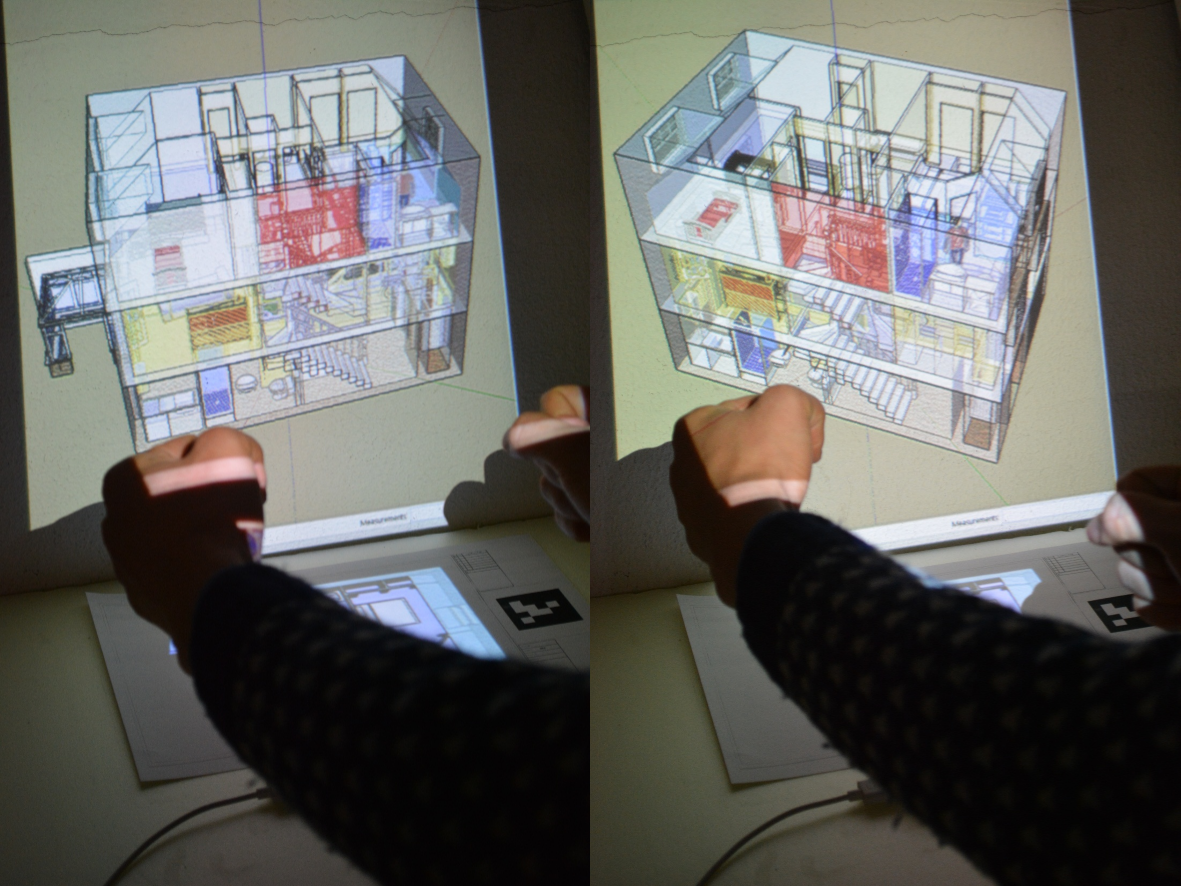
\includegraphics[width=\textwidth]{4-Interaction_Design/3d_rotate}
                \caption{Rotating the Model}
                \label{fig:rotate}
        \end{subfigure}%
        \hfill
        \begin{subfigure}[b]{0.32\textwidth}
            \centering
            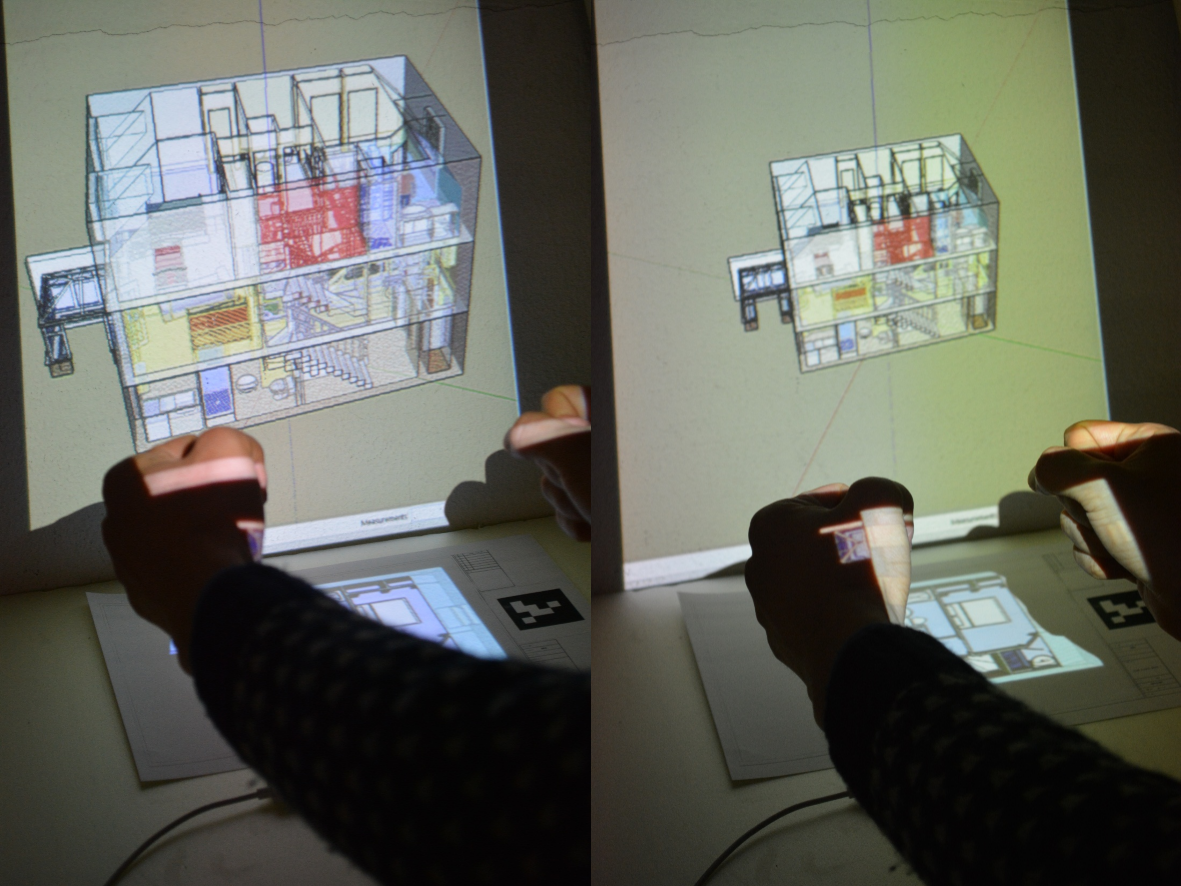
\includegraphics[width=\textwidth]{4-Interaction_Design/3d_scale_two_hand}
                \caption{Scaling by Two Hand Gesture}
                \label{fig:scale_two_hand}
        \end{subfigure}
        \hfill
        \begin{subfigure}[b]{0.32\textwidth}
            \centering
            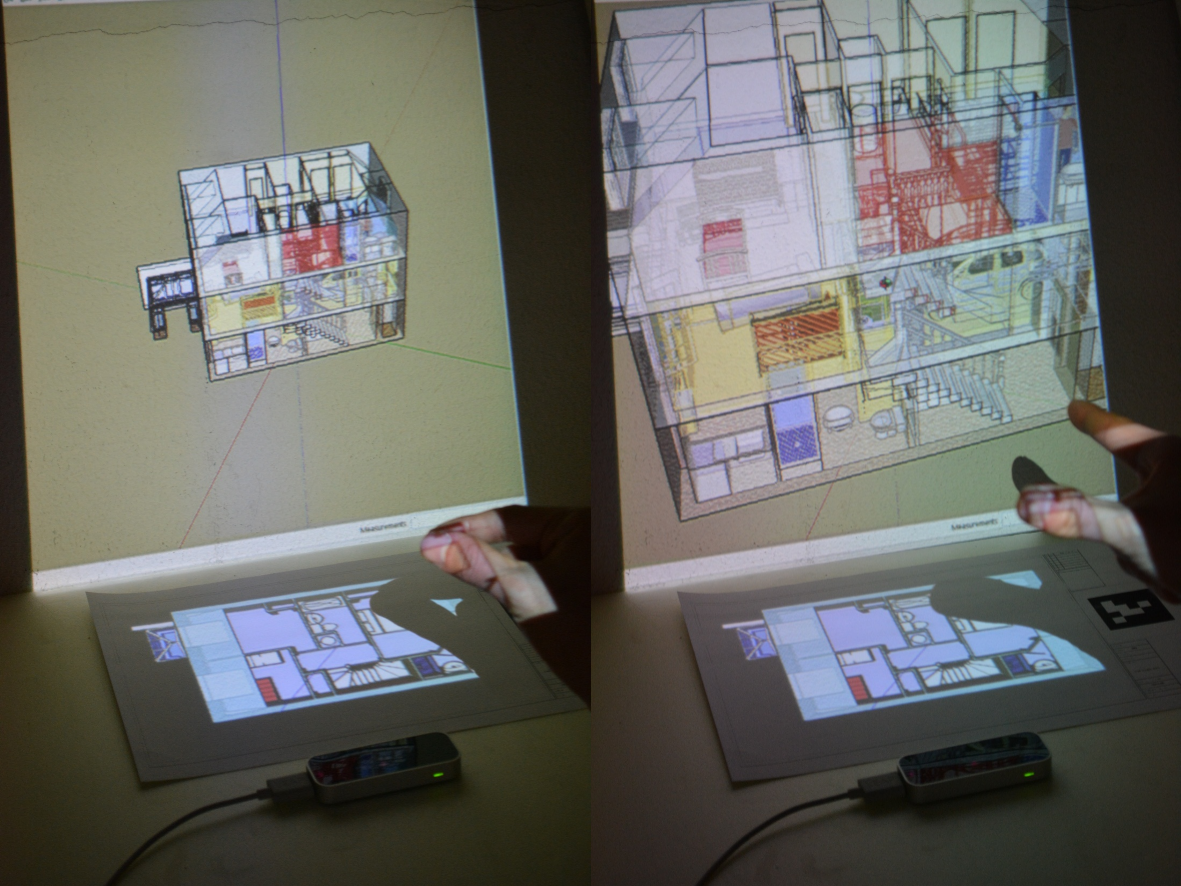
\includegraphics[width=\textwidth]{4-Interaction_Design/3d_scale_one_hand}
                \caption{Scaling by One Hand Gesture}
                \label{fig:scale_pinch}
        \end{subfigure}
	\caption{3D Manipulation}
    \label{fig:3d_mani}
\end{figure*}

사용자의 손 또는 손가락을 인식하여 3D 건축 모델의 회전 기능을 가능하게 한다. 그림 \ref{fig:rotate}처럼 사용자의 양손을 위치를 기준으로 3차원 공간에서 회전을 수행한다. 
Rotating 기능뿐만 아니라, 3D 모델을 확대하거나 축소하여 보는 Scaling 기능을 제공한다. 이 때, 직관적인 상호작용을 위하여 두 가지 모드의 Scaling 방법을 제공한다. 첫 번째 방법은, Rotating 기능과 동시에 수행할 수 있도록 양 손을 이용한 Scaling 기능을 수행 한다. 이는 그림 \ref{fig:scale_two_hand}과 같이 양손을 인식하고 거리 변화를 측정하여 3D 모델의 크기 조절을 가능하게 한다. 두 번째 방법은 그림 \ref{fig:scale_pinch}과 같이 손의 엄지와 검지 손가락을 이용하여 핀치 제스처를 인식하고 핀치 제스처의 움직임을 기반으로 3D 모델의 크기 조절이 가능하게 한다.

\subsection{Querying Specific Floor Plan}
특정 평면도의 정보에 접근할 필요가 있을 때, 그림 \ref{fig:layer}과 같이 손가락을 인식하여 평면도의 정보를 선택하여 확인 가능 하다. 시스템과 건축 모델링툴(ex, SketchUp)을 동기화하여 건물의 도면 정보를 이용하여 전체 건물 정보에서 특정 평면의 정보를 Horizontal Display에 증강 하도록 한다. 
 \begin{figure}[h!]
\centering
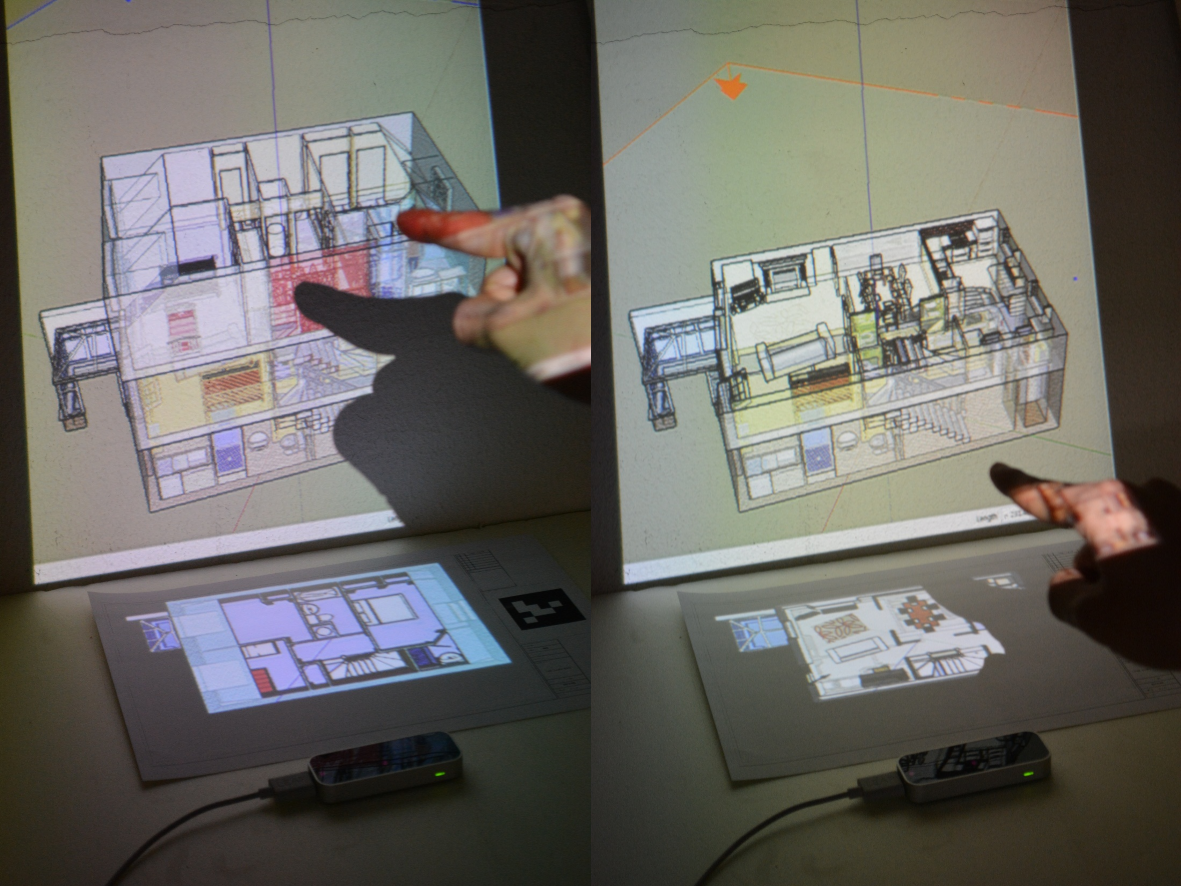
\includegraphics[width=0.4\textwidth]{4-Interaction_Design/query_plane}
\caption{Querying Specific Floor Plan}
\label{fig:layer}
\end{figure}


\subsection{Additional Information Retrieval}

또한, 취득한 도면의 부가적인 정보를 이용하여 면적이나 부피 등을 파악해야 하는 경우도 발생한다. 예를 들어 \cite{song_penlight:_2009}에서 제안한 것과 같이 건축 도면에서 부가적인 Dimension 정보를 제공하는 것은 현장에서 유용하게 사용될 수 있다. 본 연구에서는 건축 모델링툴 중 SketchUp에서 제공하는 Entity 정보를 이용하여 평면의 면적, 부피 등의 정보를 사용자에게 제공하였다. 또한 3D 정보를 제공함으로써 in-air 터치한 벽면의 넓이나 기둥의 높이 등의 3차원 Entity 정보를 제공할 수 있다. 
\begin{figure*}[!ht]
	\centering
        \begin{subfigure}[b]{0.55\textwidth}
	        \centering
                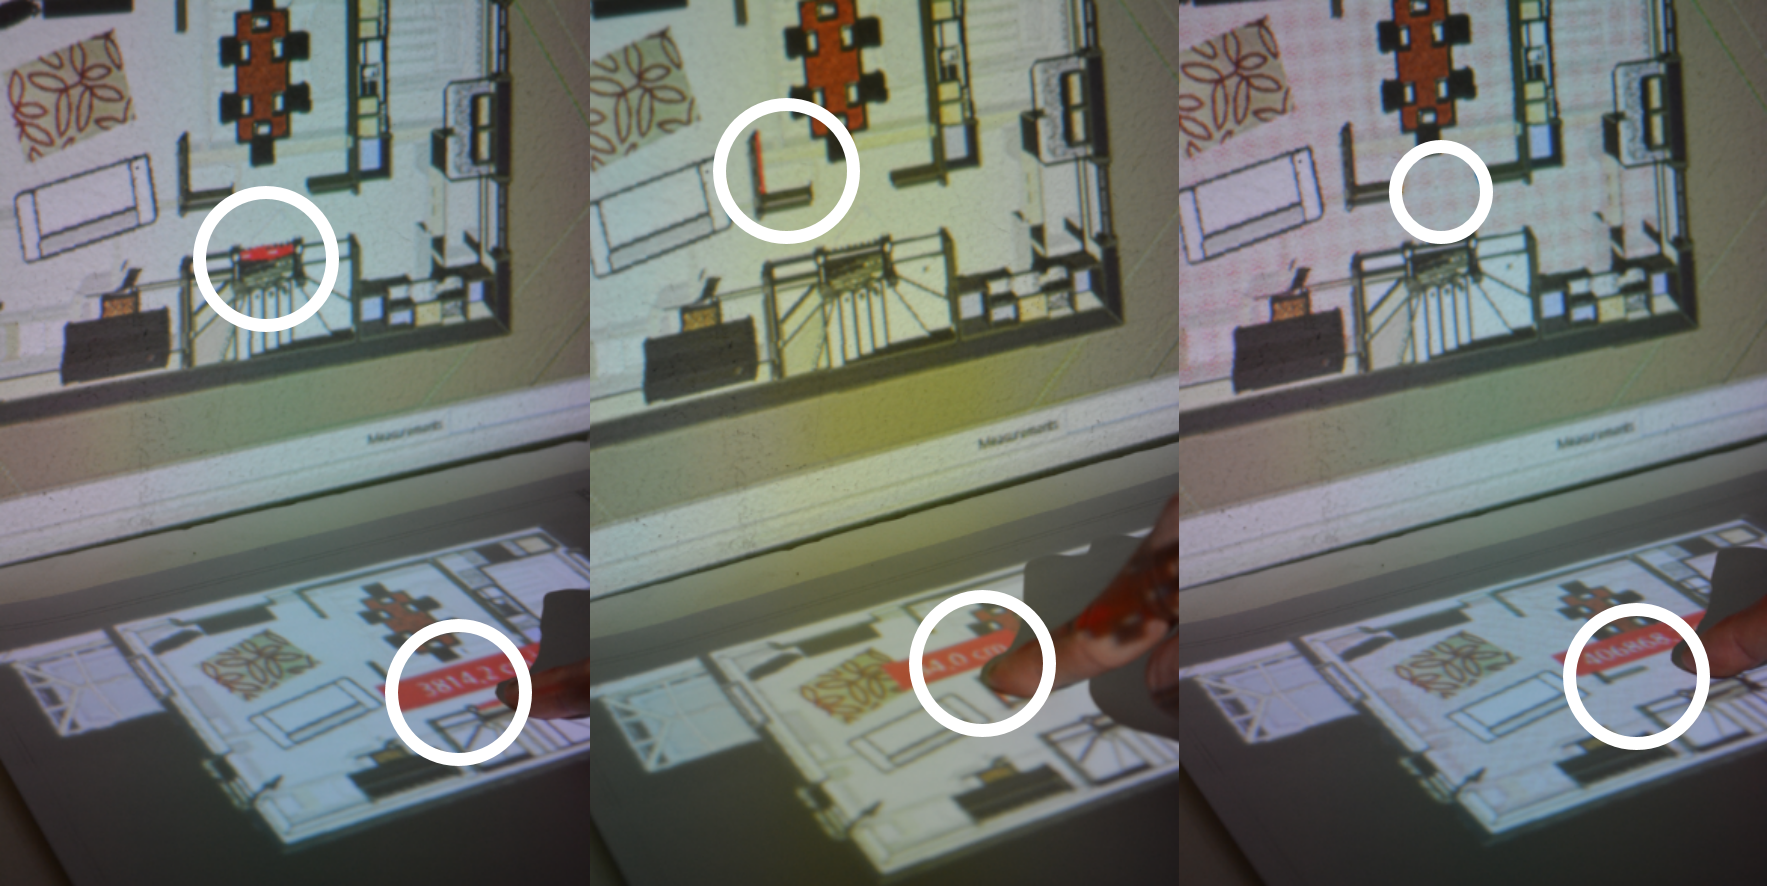
\includegraphics[width=\textwidth]{4-Interaction_Design/2d_info}
                \caption{Querying 2D information - length, area, volumn of specific entity}
                \label{fig:2d_info}
        \end{subfigure}%
        \hfill
        \begin{subfigure}[b]{0.37\textwidth}
            \centering
            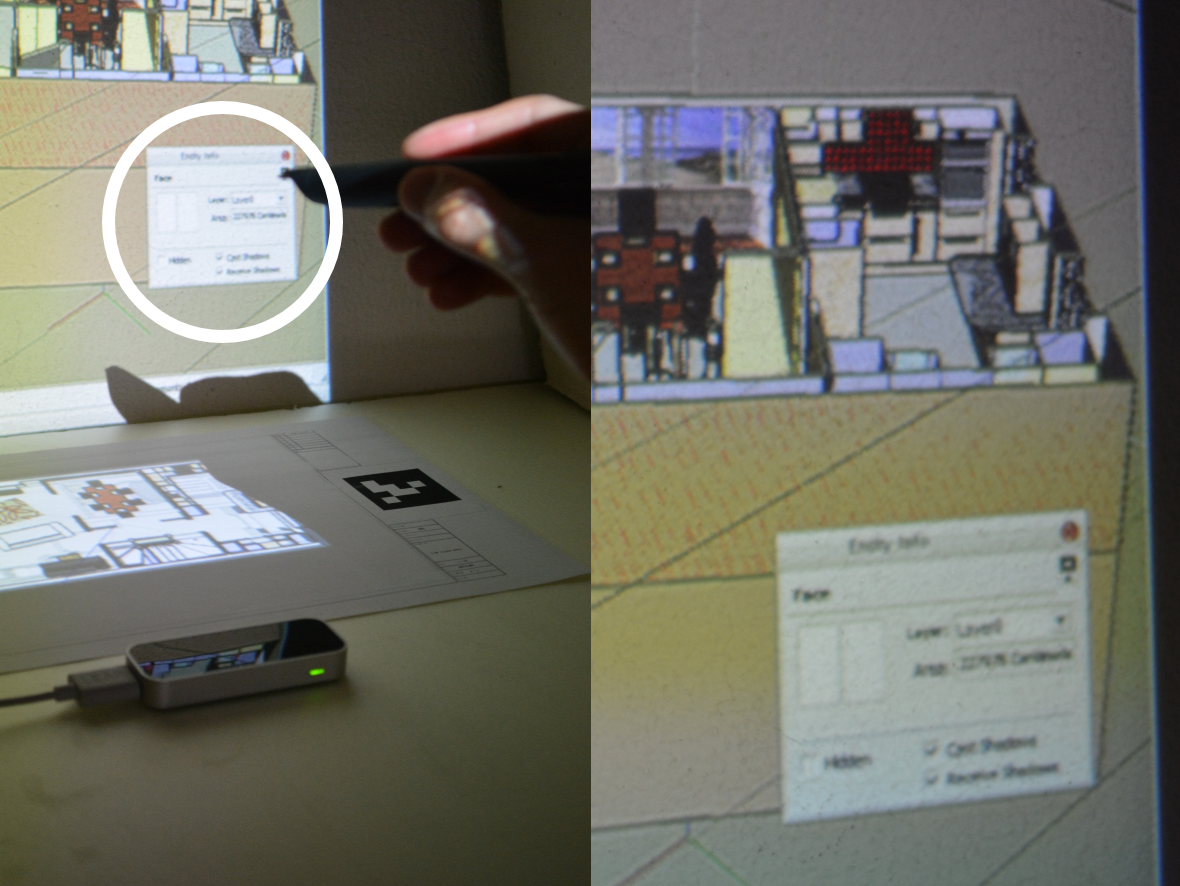
\includegraphics[width=\textwidth]{4-Interaction_Design/3d_info}
                \caption{3D information}
                \label{fig:3d_info}
        \end{subfigure}
	\caption{3D Manipulation}
    \label{fig:infor}
\end{figure*}


2D Information Retrieval
2D 정보 제공은 그림 \ref{fig:2d_info}와 같이 도면에 나타난 벽면의 길이나 바닥 면, 가구 등의 부피 등의 도면을 직접 터치함으로써 획득할 수 있다. 이는 해당 건축 도면 상에서 터치된 2차원 위치를 이용하여 시스템상의 Entity 정보를 이용하여 획득 가능하다.
3D Information Retrieval
3D 정보 제공은 그림 \ref{fig:3d_info}와 같이 제스처를 이용하여 3D 모델을 선택함으로써 정보를 제공받게 된다. 2D에 대한 정보 획득이 도면을 이용한 Horizontal Display를 이용한 입력이었다면, 3D에 대한 정보는 Vertical Display를 직접적으로 터치함으로써 입력이 제공된다. 

\subsection{On-site Editing}
현 시스템에서 도면의 변경이 필요한 경우, 정보에 대한 접근과 수정이 어렵기 때문에 변경사항을 실시간으로 반영하기 어렵다. 본 연구에서는 사용자의 손 움직임과 터치를 이용하여 건축 모델을 실시간 선택하고, 이동하거나 수정 가능하도록 하였다. 
\begin{figure}[h!]
    \centering
        \begin{subfigure}[b]{0.49\columnwidth}
            \centering
                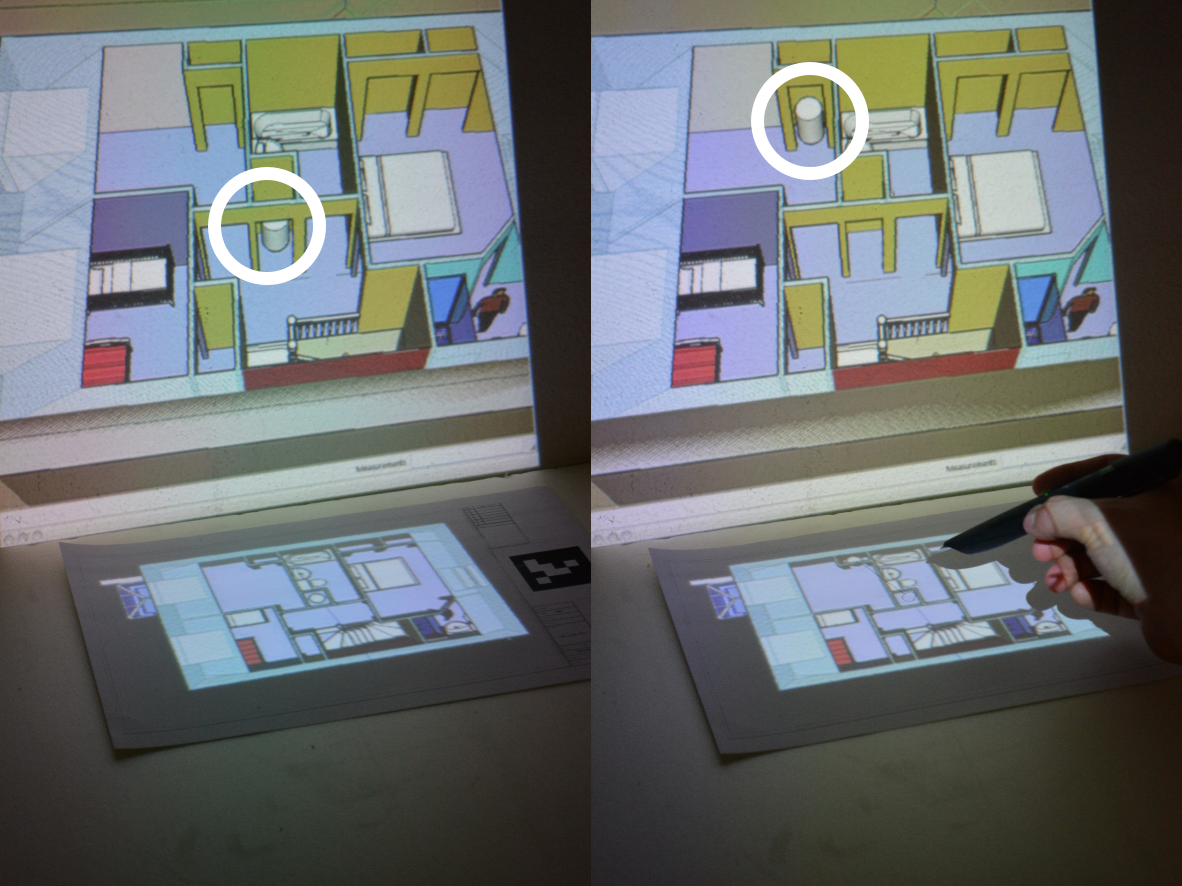
\includegraphics[width=1.0\columnwidth, height=3.6cm]{4-Interaction_Design/2d_move}
                \caption{Modifying 2D Entity using Pen}
                \label{fig:Pen_move}
        \end{subfigure}%
        \hfill
        \begin{subfigure}[b]{0.49\columnwidth}
            \centering
            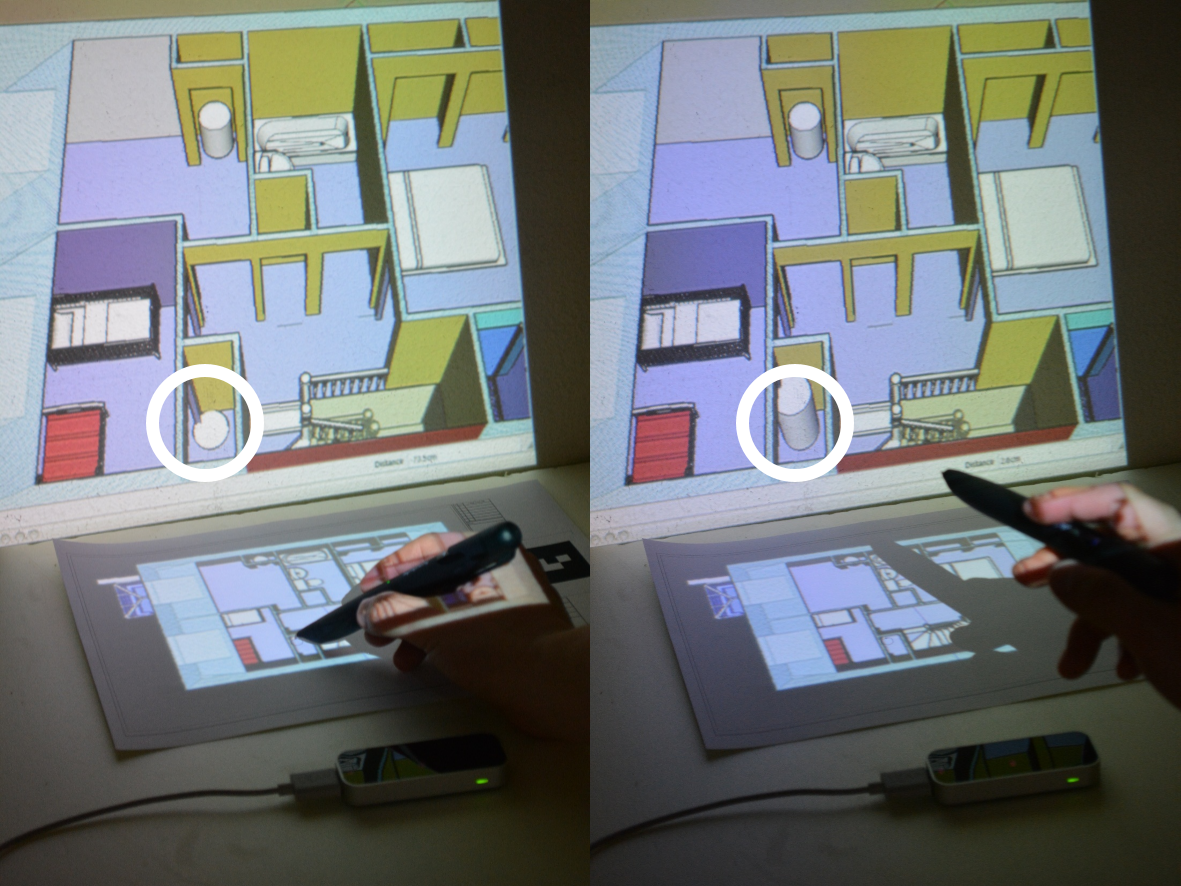
\includegraphics[width=1.0\columnwidth, height=3.6cm]{4-Interaction_Design/3d_note}
                \caption{Modifying 3D Entity in-air}
                \label{fig:Annotation}
        \end{subfigure}
    \caption{On-site Editing using Pen}
    \label{fig:edit}
\end{figure}

\textcolor{red}{제공된 컨텐츠를 정리하고, 전체적인 그림으로 표현, 삽입 예정}
